\documentclass[1p]{elsarticle_modified}
%\bibliographystyle{elsarticle-num}

%\usepackage[colorlinks]{hyperref}
%\usepackage{abbrmath_seonhwa} %\Abb, \Ascr, \Acal ,\Abf, \Afrak
\usepackage{amsfonts}
\usepackage{amssymb}
\usepackage{amsmath}
\usepackage{amsthm}
\usepackage{scalefnt}
\usepackage{amsbsy}
\usepackage{kotex}
\usepackage{caption}
\usepackage{subfig}
\usepackage{color}
\usepackage{graphicx}
\usepackage{xcolor} %% white, black, red, green, blue, cyan, magenta, yellow
\usepackage{float}
\usepackage{setspace}
\usepackage{hyperref}

\usepackage{tikz}
\usetikzlibrary{arrows}

\usepackage{multirow}
\usepackage{array} % fixed length table
\usepackage{hhline}

%%%%%%%%%%%%%%%%%%%%%
\makeatletter
\renewcommand*\env@matrix[1][\arraystretch]{%
	\edef\arraystretch{#1}%
	\hskip -\arraycolsep
	\let\@ifnextchar\new@ifnextchar
	\array{*\c@MaxMatrixCols c}}
\makeatother %https://tex.stackexchange.com/questions/14071/how-can-i-increase-the-line-spacing-in-a-matrix
%%%%%%%%%%%%%%%

\usepackage[normalem]{ulem}

\newcommand{\msout}[1]{\ifmmode\text{\sout{\ensuremath{#1}}}\else\sout{#1}\fi}
%SOURCE: \msout is \stkout macro in https://tex.stackexchange.com/questions/20609/strikeout-in-math-mode

\newcommand{\cancel}[1]{
	\ifmmode
	{\color{red}\msout{#1}}
	\else
	{\color{red}\sout{#1}}
	\fi
}

\newcommand{\add}[1]{
	{\color{blue}\uwave{#1}}
}

\newcommand{\replace}[2]{
	\ifmmode
	{\color{red}\msout{#1}}{\color{blue}\uwave{#2}}
	\else
	{\color{red}\sout{#1}}{\color{blue}\uwave{#2}}
	\fi
}

\newcommand{\Sol}{\mathcal{S}} %segment
\newcommand{\D}{D} %diagram
\newcommand{\A}{\mathcal{A}} %arc


%%%%%%%%%%%%%%%%%%%%%%%%%%%%%5 test

\def\sl{\operatorname{\textup{SL}}(2,\Cbb)}
\def\psl{\operatorname{\textup{PSL}}(2,\Cbb)}
\def\quan{\mkern 1mu \triangleright \mkern 1mu}

\theoremstyle{definition}
\newtheorem{thm}{Theorem}[section]
\newtheorem{prop}[thm]{Proposition}
\newtheorem{lem}[thm]{Lemma}
\newtheorem{ques}[thm]{Question}
\newtheorem{cor}[thm]{Corollary}
\newtheorem{defn}[thm]{Definition}
\newtheorem{exam}[thm]{Example}
\newtheorem{rmk}[thm]{Remark}
\newtheorem{alg}[thm]{Algorithm}

\newcommand{\I}{\sqrt{-1}}
\begin{document}

%\begin{frontmatter}
%
%\title{Boundary parabolic representations of knots up to 8 crossings}
%
%%% Group authors per affiliation:
%\author{Yunhi Cho} 
%\address{Department of Mathematics, University of Seoul, Seoul, Korea}
%\ead{yhcho@uos.ac.kr}
%
%
%\author{Seonhwa Kim} %\fnref{s_kim}}
%\address{Center for Geometry and Physics, Institute for Basic Science, Pohang, 37673, Korea}
%\ead{ryeona17@ibs.re.kr}
%
%\author{Hyuk Kim}
%\address{Department of Mathematical Sciences, Seoul National University, Seoul 08826, Korea}
%\ead{hyukkim@snu.ac.kr}
%
%\author{Seokbeom Yoon}
%\address{Department of Mathematical Sciences, Seoul National University, Seoul, 08826,  Korea}
%\ead{sbyoon15@snu.ac.kr}
%
%\begin{abstract}
%We find all boundary parabolic representation of knots up to 8 crossings.
%
%\end{abstract}
%\begin{keyword}
%    \MSC[2010] 57M25 
%\end{keyword}
%
%\end{frontmatter}

%\linenumbers
%\tableofcontents
%
\newcommand\colored[1]{\textcolor{white}{\rule[-0.35ex]{0.8em}{1.4ex}}\kern-0.8em\color{red} #1}%
%\newcommand\colored[1]{\textcolor{white}{ #1}\kern-2.17ex	\textcolor{white}{ #1}\kern-1.81ex	\textcolor{white}{ #1}\kern-2.15ex\color{red}#1	}

{\Large $\underline{12a_{0917}~(K12a_{0917})}$}

\setlength{\tabcolsep}{10pt}
\renewcommand{\arraystretch}{1.6}
\vspace{1cm}\begin{tabular}{m{100pt}>{\centering\arraybackslash}m{274pt}}
\multirow{5}{120pt}{
	\centering
	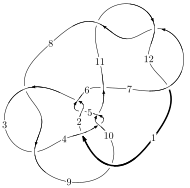
\includegraphics[width=112pt]{../../../GIT/diagram.site/Diagrams/png/1718_12a_0917.png}\\
\ \ \ A knot diagram\footnotemark}&
\allowdisplaybreaks
\textbf{Linearized knot diagam} \\
\cline{2-2}
 &
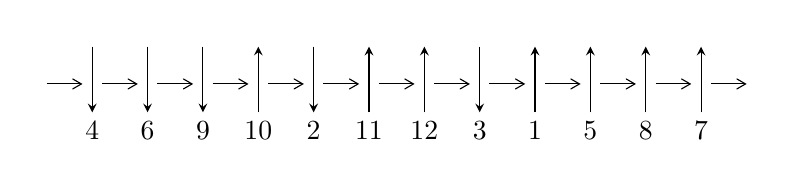
\begin{tikzpicture}[x=20pt, y=17pt]
	% nodes
	\node (C0) at (0, 0) {};
	\node (C1) at (1, 0) {};
	\node (C1U) at (1, +1) {};
	\node (C1D) at (1, -1) {4};

	\node (C2) at (2, 0) {};
	\node (C2U) at (2, +1) {};
	\node (C2D) at (2, -1) {6};

	\node (C3) at (3, 0) {};
	\node (C3U) at (3, +1) {};
	\node (C3D) at (3, -1) {9};

	\node (C4) at (4, 0) {};
	\node (C4U) at (4, +1) {};
	\node (C4D) at (4, -1) {10};

	\node (C5) at (5, 0) {};
	\node (C5U) at (5, +1) {};
	\node (C5D) at (5, -1) {2};

	\node (C6) at (6, 0) {};
	\node (C6U) at (6, +1) {};
	\node (C6D) at (6, -1) {11};

	\node (C7) at (7, 0) {};
	\node (C7U) at (7, +1) {};
	\node (C7D) at (7, -1) {12};

	\node (C8) at (8, 0) {};
	\node (C8U) at (8, +1) {};
	\node (C8D) at (8, -1) {3};

	\node (C9) at (9, 0) {};
	\node (C9U) at (9, +1) {};
	\node (C9D) at (9, -1) {1};

	\node (C10) at (10, 0) {};
	\node (C10U) at (10, +1) {};
	\node (C10D) at (10, -1) {5};

	\node (C11) at (11, 0) {};
	\node (C11U) at (11, +1) {};
	\node (C11D) at (11, -1) {8};

	\node (C12) at (12, 0) {};
	\node (C12U) at (12, +1) {};
	\node (C12D) at (12, -1) {7};
	\node (C13) at (13, 0) {};

	% arrows
	\draw[->,>={angle 60}]
	(C0) edge (C1) (C1) edge (C2) (C2) edge (C3) (C3) edge (C4) (C4) edge (C5) (C5) edge (C6) (C6) edge (C7) (C7) edge (C8) (C8) edge (C9) (C9) edge (C10) (C10) edge (C11) (C11) edge (C12) (C12) edge (C13) ;	\draw[->,>=stealth]
	(C1U) edge (C1D) (C2U) edge (C2D) (C3U) edge (C3D) (C4D) edge (C4U) (C5U) edge (C5D) (C6D) edge (C6U) (C7D) edge (C7U) (C8U) edge (C8D) (C9D) edge (C9U) (C10D) edge (C10U) (C11D) edge (C11U) (C12D) edge (C12U) ;
	\end{tikzpicture} \\
\hhline{~~} \\& 
\textbf{Solving Sequence} \\ \cline{2-2} 
 &
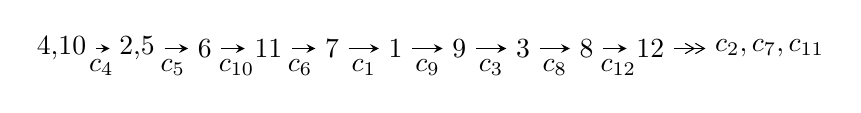
\begin{tikzpicture}[x=23pt, y=7pt]
	% node
	\node (A0) at (-1/8, 0) {4,10};
	\node (A1) at (17/16, 0) {2,5};
	\node (A2) at (17/8, 0) {6};
	\node (A3) at (25/8, 0) {11};
	\node (A4) at (33/8, 0) {7};
	\node (A5) at (41/8, 0) {1};
	\node (A6) at (49/8, 0) {9};
	\node (A7) at (57/8, 0) {3};
	\node (A8) at (65/8, 0) {8};
	\node (A9) at (73/8, 0) {12};
	\node (C1) at (1/2, -1) {$c_{4}$};
	\node (C2) at (13/8, -1) {$c_{5}$};
	\node (C3) at (21/8, -1) {$c_{10}$};
	\node (C4) at (29/8, -1) {$c_{6}$};
	\node (C5) at (37/8, -1) {$c_{1}$};
	\node (C6) at (45/8, -1) {$c_{9}$};
	\node (C7) at (53/8, -1) {$c_{3}$};
	\node (C8) at (61/8, -1) {$c_{8}$};
	\node (C9) at (69/8, -1) {$c_{12}$};
	\node (A10) at (11, 0) {$c_{2},c_{7},c_{11}$};

	% edge
	\draw[->,>=stealth]	
	(A0) edge (A1) (A1) edge (A2) (A2) edge (A3) (A3) edge (A4) (A4) edge (A5) (A5) edge (A6) (A6) edge (A7) (A7) edge (A8) (A8) edge (A9) ;
	\draw[->>,>={angle 60}]	
	(A9) edge (A10);
\end{tikzpicture} \\ 

\end{tabular} \\

\footnotetext{
The image of knot diagram is generated by the software ``\textbf{Draw programme}" developed by Andrew Bartholomew(\url{http://www.layer8.co.uk/maths/draw/index.htm\#Running-draw}), where we modified some parts for our purpose(\url{https://github.com/CATsTAILs/LinksPainter}).
}\phantom \\ \newline 
\centering \textbf{Ideals for irreducible components\footnotemark of $X_{\text{par}}$} 
 
\begin{align*}
I^u_{1}&=\langle 
-3.88633\times10^{471} u^{113}+1.54579\times10^{470} u^{112}+\cdots+7.97071\times10^{471} b+1.97275\times10^{474},\\
\phantom{I^u_{1}}&\phantom{= \langle  }7.18453\times10^{474} u^{113}+6.27512\times10^{473} u^{112}+\cdots+5.89036\times10^{474} a-5.31194\times10^{477},\\
\phantom{I^u_{1}}&\phantom{= \langle  }u^{114}- u^{113}+\cdots+3336 u+739\rangle \\
I^u_{2}&=\langle 
u^{17}- u^{15}+u^{14}-2 u^{13}- u^{12}+4 u^{11}-2 u^{10}+u^8-5 u^7+2 u^5-2 u^4+2 u^3- u^2+b- u,\\
\phantom{I^u_{2}}&\phantom{= \langle  }-2 u^{17}+3 u^{16}+\cdots+a-8,\\
\phantom{I^u_{2}}&\phantom{= \langle  }u^{18}-2 u^{16}+u^{15}- u^{14}-2 u^{13}+6 u^{12}- u^{11}-4 u^{10}+3 u^9-5 u^8- u^7+7 u^6-2 u^5+u^3-3 u^2+1\rangle \\
\\
\end{align*}
\raggedright * 2 irreducible components of $\dim_{\mathbb{C}}=0$, with total 132 representations.\\
\footnotetext{All coefficients of polynomials are rational numbers. But the coefficients are sometimes approximated in decimal forms when there is not enough margin.}
\newpage
\renewcommand{\arraystretch}{1}
\centering \section*{I. $I^u_{1}= \langle -3.89\times10^{471} u^{113}+1.55\times10^{470} u^{112}+\cdots+7.97\times10^{471} b+1.97\times10^{474},\;7.18\times10^{474} u^{113}+6.28\times10^{473} u^{112}+\cdots+5.89\times10^{474} a-5.31\times10^{477},\;u^{114}- u^{113}+\cdots+3336 u+739 \rangle$}
\flushleft \textbf{(i) Arc colorings}\\
\begin{tabular}{m{7pt} m{180pt} m{7pt} m{180pt} }
\flushright $a_{4}=$&$\begin{pmatrix}1\\0\end{pmatrix}$ \\
\flushright $a_{10}=$&$\begin{pmatrix}0\\u\end{pmatrix}$ \\
\flushright $a_{2}=$&$\begin{pmatrix}-1.21971 u^{113}-0.106532 u^{112}+\cdots+4748.64 u+901.802\\0.487577 u^{113}-0.0193933 u^{112}+\cdots-1361.90 u-247.500\end{pmatrix}$ \\
\flushright $a_{5}=$&$\begin{pmatrix}1\\- u^2\end{pmatrix}$ \\
\flushright $a_{6}=$&$\begin{pmatrix}-0.702049 u^{113}-0.0653924 u^{112}+\cdots+3470.05 u+644.021\\0.845663 u^{113}-0.192654 u^{112}+\cdots-3774.60 u-650.263\end{pmatrix}$ \\
\flushright $a_{11}=$&$\begin{pmatrix}u\\- u^3+u\end{pmatrix}$ \\
\flushright $a_{7}=$&$\begin{pmatrix}-0.0422999 u^{113}-0.195938 u^{112}+\cdots+427.605 u+115.860\\1.02739 u^{113}-0.224671 u^{112}+\cdots-4564.07 u-787.343\end{pmatrix}$ \\
\flushright $a_{1}=$&$\begin{pmatrix}-0.732134 u^{113}-0.125925 u^{112}+\cdots+3386.74 u+654.302\\0.487577 u^{113}-0.0193933 u^{112}+\cdots-1361.90 u-247.500\end{pmatrix}$ \\
\flushright $a_{9}=$&$\begin{pmatrix}0.168656 u^{113}-0.108635 u^{112}+\cdots+315.475 u+96.2647\\-0.565787 u^{113}+0.0498570 u^{112}+\cdots+2951.46 u+531.758\end{pmatrix}$ \\
\flushright $a_{3}=$&$\begin{pmatrix}-0.444496 u^{113}+0.325385 u^{112}+\cdots+1254.43 u+185.049\\0.196882 u^{113}+0.141099 u^{112}+\cdots-654.563 u-145.912\end{pmatrix}$ \\
\flushright $a_{8}=$&$\begin{pmatrix}-0.393672 u^{113}+0.129234 u^{112}+\cdots+1069.44 u+180.809\\-0.748105 u^{113}+0.105672 u^{112}+\cdots+2739.36 u+481.056\end{pmatrix}$ \\
\flushright $a_{12}=$&$\begin{pmatrix}0.316425 u^{113}-0.0597294 u^{112}+\cdots-1059.92 u-181.231\\0.570528 u^{113}-0.0518741 u^{112}+\cdots-2263.23 u-397.890\end{pmatrix}$\\&\end{tabular}
\flushleft \textbf{(ii) Obstruction class $= -1$}\\~\\
\flushleft \textbf{(iii) Cusp Shapes $= 0.538110 u^{113}-0.379647 u^{112}+\cdots-40.7556 u+70.1323$}\\~\\
\newpage\renewcommand{\arraystretch}{1}
\flushleft \textbf{(iv) u-Polynomials at the component}\newline \\
\begin{tabular}{m{50pt}|m{274pt}}
Crossings & \hspace{64pt}u-Polynomials at each crossing \\
\hline $$\begin{aligned}c_{1}\end{aligned}$$&$\begin{aligned}
&u^{114}-4 u^{113}+\cdots-26 u+1
\end{aligned}$\\
\hline $$\begin{aligned}c_{2},c_{5}\end{aligned}$$&$\begin{aligned}
&u^{114}+u^{113}+\cdots-712 u-329
\end{aligned}$\\
\hline $$\begin{aligned}c_{3},c_{8}\end{aligned}$$&$\begin{aligned}
&u^{114}+u^{113}+\cdots+35970 u+3559
\end{aligned}$\\
\hline $$\begin{aligned}c_{4},c_{10}\end{aligned}$$&$\begin{aligned}
&u^{114}- u^{113}+\cdots+3336 u+739
\end{aligned}$\\
\hline $$\begin{aligned}c_{6}\end{aligned}$$&$\begin{aligned}
&u^{114}+u^{113}+\cdots+57678 u-19897
\end{aligned}$\\
\hline $$\begin{aligned}c_{7},c_{11},c_{12}\end{aligned}$$&$\begin{aligned}
&u^{114}- u^{113}+\cdots+12 u-1
\end{aligned}$\\
\hline $$\begin{aligned}c_{9}\end{aligned}$$&$\begin{aligned}
&u^{114}-2 u^{113}+\cdots-2 u+1
\end{aligned}$\\
\hline
\end{tabular}\\~\\
\newpage\renewcommand{\arraystretch}{1}
\flushleft \textbf{(v) Riley Polynomials at the component}\newline \\
\begin{tabular}{m{50pt}|m{274pt}}
Crossings & \hspace{64pt}Riley Polynomials at each crossing \\
\hline $$\begin{aligned}c_{1}\end{aligned}$$&$\begin{aligned}
&y^{114}-16 y^{113}+\cdots-48 y+1
\end{aligned}$\\
\hline $$\begin{aligned}c_{2},c_{5}\end{aligned}$$&$\begin{aligned}
&y^{114}-77 y^{113}+\cdots-6990876 y+108241
\end{aligned}$\\
\hline $$\begin{aligned}c_{3},c_{8}\end{aligned}$$&$\begin{aligned}
&y^{114}-73 y^{113}+\cdots-385996944 y+12666481
\end{aligned}$\\
\hline $$\begin{aligned}c_{4},c_{10}\end{aligned}$$&$\begin{aligned}
&y^{114}-63 y^{113}+\cdots-24991058 y+546121
\end{aligned}$\\
\hline $$\begin{aligned}c_{6}\end{aligned}$$&$\begin{aligned}
&y^{114}-13 y^{113}+\cdots-36931949010 y+395890609
\end{aligned}$\\
\hline $$\begin{aligned}c_{7},c_{11},c_{12}\end{aligned}$$&$\begin{aligned}
&y^{114}+103 y^{113}+\cdots-100 y+1
\end{aligned}$\\
\hline $$\begin{aligned}c_{9}\end{aligned}$$&$\begin{aligned}
&y^{114}-10 y^{113}+\cdots-56 y+1
\end{aligned}$\\
\hline
\end{tabular}\\~\\
\newpage\flushleft \textbf{(vi) Complex Volumes and Cusp Shapes}
$$\begin{array}{c|c|c}  
\text{Solutions to }I^u_{1}& \I (\text{vol} + \sqrt{-1}CS) & \text{Cusp shape}\\
 \hline 
\begin{aligned}
u &= -0.969088 + 0.204379 I \\
a &= \phantom{-}0.414722 - 0.810630 I \\
b &= -1.42649 + 0.70549 I\end{aligned}
 & -3.50634 - 4.69984 I & \phantom{-0.000000 } 0 \\ \hline\begin{aligned}
u &= -0.969088 - 0.204379 I \\
a &= \phantom{-}0.414722 + 0.810630 I \\
b &= -1.42649 - 0.70549 I\end{aligned}
 & -3.50634 + 4.69984 I & \phantom{-0.000000 } 0 \\ \hline\begin{aligned}
u &= \phantom{-}0.877583 + 0.445562 I \\
a &= -0.21000 + 1.84305 I \\
b &= \phantom{-}0.358065 + 0.009637 I\end{aligned}
 & -2.36151 + 5.03253 I & \phantom{-0.000000 } 0 \\ \hline\begin{aligned}
u &= \phantom{-}0.877583 - 0.445562 I \\
a &= -0.21000 - 1.84305 I \\
b &= \phantom{-}0.358065 - 0.009637 I\end{aligned}
 & -2.36151 - 5.03253 I & \phantom{-0.000000 } 0 \\ \hline\begin{aligned}
u &= -0.006438 + 1.028020 I \\
a &= -0.155991 + 0.265312 I \\
b &= \phantom{-}1.074920 + 0.501547 I\end{aligned}
 & -6.60704 - 3.50811 I & \phantom{-0.000000 } 0 \\ \hline\begin{aligned}
u &= -0.006438 - 1.028020 I \\
a &= -0.155991 - 0.265312 I \\
b &= \phantom{-}1.074920 - 0.501547 I\end{aligned}
 & -6.60704 + 3.50811 I & \phantom{-0.000000 } 0 \\ \hline\begin{aligned}
u &= -0.695698 + 0.757499 I \\
a &= \phantom{-}0.452586 - 0.492180 I \\
b &= \phantom{-}0.345815 + 0.231181 I\end{aligned}
 & -3.24887 - 2.33723 I & \phantom{-0.000000 } 0 \\ \hline\begin{aligned}
u &= -0.695698 - 0.757499 I \\
a &= \phantom{-}0.452586 + 0.492180 I \\
b &= \phantom{-}0.345815 - 0.231181 I\end{aligned}
 & -3.24887 + 2.33723 I & \phantom{-0.000000 } 0 \\ \hline\begin{aligned}
u &= \phantom{-}0.968126 + 0.073076 I \\
a &= \phantom{-}0.650180 + 1.183770 I \\
b &= -1.58042 - 0.93058 I\end{aligned}
 & \phantom{-}1.51276 + 0.70933 I & \phantom{-0.000000 } 0 \\ \hline\begin{aligned}
u &= \phantom{-}0.968126 - 0.073076 I \\
a &= \phantom{-}0.650180 - 1.183770 I \\
b &= -1.58042 + 0.93058 I\end{aligned}
 & \phantom{-}1.51276 - 0.70933 I & \phantom{-0.000000 } 0\\
 \hline 
 \end{array}$$\newpage$$\begin{array}{c|c|c}  
\text{Solutions to }I^u_{1}& \I (\text{vol} + \sqrt{-1}CS) & \text{Cusp shape}\\
 \hline 
\begin{aligned}
u &= \phantom{-}0.949489 + 0.055564 I \\
a &= \phantom{-}0.55669 - 1.61663 I \\
b &= \phantom{-}0.061562 + 0.974667 I\end{aligned}
 & \phantom{-}1.41876 + 0.03926 I & \phantom{-0.000000 } 0 \\ \hline\begin{aligned}
u &= \phantom{-}0.949489 - 0.055564 I \\
a &= \phantom{-}0.55669 + 1.61663 I \\
b &= \phantom{-}0.061562 - 0.974667 I\end{aligned}
 & \phantom{-}1.41876 - 0.03926 I & \phantom{-0.000000 } 0 \\ \hline\begin{aligned}
u &= \phantom{-}0.954829 + 0.446281 I \\
a &= -0.06902 - 2.04103 I \\
b &= -0.582983 + 0.860904 I\end{aligned}
 & -5.06278 + 6.04773 I & \phantom{-0.000000 } 0 \\ \hline\begin{aligned}
u &= \phantom{-}0.954829 - 0.446281 I \\
a &= -0.06902 + 2.04103 I \\
b &= -0.582983 - 0.860904 I\end{aligned}
 & -5.06278 - 6.04773 I & \phantom{-0.000000 } 0 \\ \hline\begin{aligned}
u &= \phantom{-}0.914791 + 0.236855 I \\
a &= -1.58640 + 1.57134 I \\
b &= \phantom{-}0.297054 + 0.009562 I\end{aligned}
 & -9.57486 - 0.48554 I & \phantom{-0.000000 } 0 \\ \hline\begin{aligned}
u &= \phantom{-}0.914791 - 0.236855 I \\
a &= -1.58640 - 1.57134 I \\
b &= \phantom{-}0.297054 - 0.009562 I\end{aligned}
 & -9.57486 + 0.48554 I & \phantom{-0.000000 } 0 \\ \hline\begin{aligned}
u &= \phantom{-}0.922232 + 0.144218 I \\
a &= \phantom{-}1.174010 - 0.065866 I \\
b &= \phantom{-}1.123630 - 0.011538 I\end{aligned}
 & -9.76533 + 2.14261 I & \phantom{-0.000000 } 0 \\ \hline\begin{aligned}
u &= \phantom{-}0.922232 - 0.144218 I \\
a &= \phantom{-}1.174010 + 0.065866 I \\
b &= \phantom{-}1.123630 + 0.011538 I\end{aligned}
 & -9.76533 - 2.14261 I & \phantom{-0.000000 } 0 \\ \hline\begin{aligned}
u &= \phantom{-}1.046070 + 0.239058 I \\
a &= -0.85138 - 1.97274 I \\
b &= \phantom{-}1.09363 + 2.03591 I\end{aligned}
 & -5.37492 + 8.65829 I & \phantom{-0.000000 } 0 \\ \hline\begin{aligned}
u &= \phantom{-}1.046070 - 0.239058 I \\
a &= -0.85138 + 1.97274 I \\
b &= \phantom{-}1.09363 - 2.03591 I\end{aligned}
 & -5.37492 - 8.65829 I & \phantom{-0.000000 } 0\\
 \hline 
 \end{array}$$\newpage$$\begin{array}{c|c|c}  
\text{Solutions to }I^u_{1}& \I (\text{vol} + \sqrt{-1}CS) & \text{Cusp shape}\\
 \hline 
\begin{aligned}
u &= -0.264647 + 0.883793 I \\
a &= -0.536581 - 0.273213 I \\
b &= \phantom{-}1.216060 - 0.609753 I\end{aligned}
 & -13.92120 + 2.15412 I & \phantom{-0.000000 } 0 \\ \hline\begin{aligned}
u &= -0.264647 - 0.883793 I \\
a &= -0.536581 + 0.273213 I \\
b &= \phantom{-}1.216060 + 0.609753 I\end{aligned}
 & -13.92120 - 2.15412 I & \phantom{-0.000000 } 0 \\ \hline\begin{aligned}
u &= -1.010120 + 0.380788 I \\
a &= -0.68331 - 1.26299 I \\
b &= \phantom{-}0.318750 + 0.019761 I\end{aligned}
 & -3.47032 - 1.40711 I & \phantom{-0.000000 } 0 \\ \hline\begin{aligned}
u &= -1.010120 - 0.380788 I \\
a &= -0.68331 + 1.26299 I \\
b &= \phantom{-}0.318750 - 0.019761 I\end{aligned}
 & -3.47032 + 1.40711 I & \phantom{-0.000000 } 0 \\ \hline\begin{aligned}
u &= -0.817063 + 0.423429 I \\
a &= -0.16216 - 2.30139 I \\
b &= \phantom{-}0.353188 - 0.037404 I\end{aligned}
 & -7.84408 - 8.47218 I & \phantom{-0.000000 } 0 \\ \hline\begin{aligned}
u &= -0.817063 - 0.423429 I \\
a &= -0.16216 + 2.30139 I \\
b &= \phantom{-}0.353188 + 0.037404 I\end{aligned}
 & -7.84408 + 8.47218 I & \phantom{-0.000000 } 0 \\ \hline\begin{aligned}
u &= -0.746591 + 0.520694 I \\
a &= \phantom{-}0.950966 + 0.221898 I \\
b &= \phantom{-}1.073110 + 0.087222 I\end{aligned}
 & -8.00719 + 4.52766 I & \phantom{-0.000000 } 0 \\ \hline\begin{aligned}
u &= -0.746591 - 0.520694 I \\
a &= \phantom{-}0.950966 - 0.221898 I \\
b &= \phantom{-}1.073110 - 0.087222 I\end{aligned}
 & -8.00719 - 4.52766 I & \phantom{-0.000000 } 0 \\ \hline\begin{aligned}
u &= -0.902077 + 0.094311 I \\
a &= \phantom{-}0.12308 + 2.02544 I \\
b &= -1.11520 - 1.36298 I\end{aligned}
 & -0.19599 - 3.84624 I & \phantom{-0.000000 } 0 \\ \hline\begin{aligned}
u &= -0.902077 - 0.094311 I \\
a &= \phantom{-}0.12308 - 2.02544 I \\
b &= -1.11520 + 1.36298 I\end{aligned}
 & -0.19599 + 3.84624 I & \phantom{-0.000000 } 0\\
 \hline 
 \end{array}$$\newpage$$\begin{array}{c|c|c}  
\text{Solutions to }I^u_{1}& \I (\text{vol} + \sqrt{-1}CS) & \text{Cusp shape}\\
 \hline 
\begin{aligned}
u &= -1.086250 + 0.162157 I \\
a &= \phantom{-}0.06438 + 2.12014 I \\
b &= \phantom{-}0.14911 - 1.94929 I\end{aligned}
 & \phantom{-}1.30462 - 4.38742 I & \phantom{-0.000000 } 0 \\ \hline\begin{aligned}
u &= -1.086250 - 0.162157 I \\
a &= \phantom{-}0.06438 - 2.12014 I \\
b &= \phantom{-}0.14911 + 1.94929 I\end{aligned}
 & \phantom{-}1.30462 + 4.38742 I & \phantom{-0.000000 } 0 \\ \hline\begin{aligned}
u &= -1.035270 + 0.478756 I \\
a &= -0.30223 + 1.61442 I \\
b &= -0.806669 - 0.959995 I\end{aligned}
 & \phantom{-}0.34780 - 4.65325 I & \phantom{-0.000000 } 0 \\ \hline\begin{aligned}
u &= -1.035270 - 0.478756 I \\
a &= -0.30223 - 1.61442 I \\
b &= -0.806669 + 0.959995 I\end{aligned}
 & \phantom{-}0.34780 + 4.65325 I & \phantom{-0.000000 } 0 \\ \hline\begin{aligned}
u &= -1.117830 + 0.247816 I \\
a &= -0.20281 + 1.52575 I \\
b &= -1.04943 - 0.98275 I\end{aligned}
 & \phantom{-}0.41343 - 3.70509 I & \phantom{-0.000000 } 0 \\ \hline\begin{aligned}
u &= -1.117830 - 0.247816 I \\
a &= -0.20281 - 1.52575 I \\
b &= -1.04943 + 0.98275 I\end{aligned}
 & \phantom{-}0.41343 + 3.70509 I & \phantom{-0.000000 } 0 \\ \hline\begin{aligned}
u &= -0.847341\phantom{ +0.000000I} \\
a &= \phantom{-}1.23534\phantom{ +0.000000I} \\
b &= \phantom{-}1.13631\phantom{ +0.000000I}\end{aligned}
 & -5.38924\phantom{ +0.000000I} & \phantom{-0.000000 } 0 \\ \hline\begin{aligned}
u &= -0.329500 + 0.765976 I \\
a &= \phantom{-}0.326623 + 0.507359 I \\
b &= \phantom{-}1.100880 + 0.290094 I\end{aligned}
 & -5.80128 - 3.00091 I & \phantom{-0.000000 } 0 \\ \hline\begin{aligned}
u &= -0.329500 - 0.765976 I \\
a &= \phantom{-}0.326623 - 0.507359 I \\
b &= \phantom{-}1.100880 - 0.290094 I\end{aligned}
 & -5.80128 + 3.00091 I & \phantom{-0.000000 } 0 \\ \hline\begin{aligned}
u &= \phantom{-}0.618576 + 0.540685 I \\
a &= \phantom{-}0.083599 + 0.252147 I \\
b &= -1.052880 - 0.515640 I\end{aligned}
 & -6.05839 - 2.02378 I & \phantom{-0.000000 } 0\\
 \hline 
 \end{array}$$\newpage$$\begin{array}{c|c|c}  
\text{Solutions to }I^u_{1}& \I (\text{vol} + \sqrt{-1}CS) & \text{Cusp shape}\\
 \hline 
\begin{aligned}
u &= \phantom{-}0.618576 - 0.540685 I \\
a &= \phantom{-}0.083599 - 0.252147 I \\
b &= -1.052880 + 0.515640 I\end{aligned}
 & -6.05839 + 2.02378 I & \phantom{-0.000000 } 0 \\ \hline\begin{aligned}
u &= \phantom{-}0.584109 + 0.576538 I \\
a &= \phantom{-}0.809406 - 0.387011 I \\
b &= \phantom{-}1.091560 - 0.150137 I\end{aligned}
 & -3.16752 - 0.88507 I & \phantom{-0.000000 } 0 \\ \hline\begin{aligned}
u &= \phantom{-}0.584109 - 0.576538 I \\
a &= \phantom{-}0.809406 + 0.387011 I \\
b &= \phantom{-}1.091560 + 0.150137 I\end{aligned}
 & -3.16752 + 0.88507 I & \phantom{-0.000000 } 0 \\ \hline\begin{aligned}
u &= -0.045428 + 1.189570 I \\
a &= -0.167656 - 0.108204 I \\
b &= \phantom{-}1.009570 - 0.563654 I\end{aligned}
 & -4.97274 + 7.84212 I & \phantom{-0.000000 } 0 \\ \hline\begin{aligned}
u &= -0.045428 - 1.189570 I \\
a &= -0.167656 + 0.108204 I \\
b &= \phantom{-}1.009570 + 0.563654 I\end{aligned}
 & -4.97274 - 7.84212 I & \phantom{-0.000000 } 0 \\ \hline\begin{aligned}
u &= -1.165720 + 0.323722 I \\
a &= \phantom{-}0.31893 + 1.56945 I \\
b &= -0.694903 - 1.156700 I\end{aligned}
 & \phantom{-}0.94177 - 4.19901 I & \phantom{-0.000000 } 0 \\ \hline\begin{aligned}
u &= -1.165720 - 0.323722 I \\
a &= \phantom{-}0.31893 - 1.56945 I \\
b &= -0.694903 + 1.156700 I\end{aligned}
 & \phantom{-}0.94177 + 4.19901 I & \phantom{-0.000000 } 0 \\ \hline\begin{aligned}
u &= \phantom{-}1.109390 + 0.508395 I \\
a &= -0.43713 - 1.64769 I \\
b &= -0.859732 + 0.839961 I\end{aligned}
 & -4.47538 + 3.22869 I & \phantom{-0.000000 } 0 \\ \hline\begin{aligned}
u &= \phantom{-}1.109390 - 0.508395 I \\
a &= -0.43713 + 1.64769 I \\
b &= -0.859732 - 0.839961 I\end{aligned}
 & -4.47538 - 3.22869 I & \phantom{-0.000000 } 0 \\ \hline\begin{aligned}
u &= \phantom{-}0.232527 + 0.731714 I \\
a &= -0.488149 + 0.051820 I \\
b &= -0.795646 - 0.709438 I\end{aligned}
 & -6.98909 + 1.36802 I & \phantom{-0.000000 } 0\\
 \hline 
 \end{array}$$\newpage$$\begin{array}{c|c|c}  
\text{Solutions to }I^u_{1}& \I (\text{vol} + \sqrt{-1}CS) & \text{Cusp shape}\\
 \hline 
\begin{aligned}
u &= \phantom{-}0.232527 - 0.731714 I \\
a &= -0.488149 - 0.051820 I \\
b &= -0.795646 + 0.709438 I\end{aligned}
 & -6.98909 - 1.36802 I & \phantom{-0.000000 } 0 \\ \hline\begin{aligned}
u &= \phantom{-}1.245280 + 0.019562 I \\
a &= \phantom{-}1.06744 - 0.93533 I \\
b &= -1.23246 + 0.91844 I\end{aligned}
 & \phantom{-}2.68980 - 0.40449 I & \phantom{-0.000000 } 0 \\ \hline\begin{aligned}
u &= \phantom{-}1.245280 - 0.019562 I \\
a &= \phantom{-}1.06744 + 0.93533 I \\
b &= -1.23246 - 0.91844 I\end{aligned}
 & \phantom{-}2.68980 + 0.40449 I & \phantom{-0.000000 } 0 \\ \hline\begin{aligned}
u &= \phantom{-}1.202270 + 0.346526 I \\
a &= -0.33320 - 1.47123 I \\
b &= -1.010690 + 0.890754 I\end{aligned}
 & \phantom{-}2.71109 + 7.20053 I & \phantom{-0.000000 } 0 \\ \hline\begin{aligned}
u &= \phantom{-}1.202270 - 0.346526 I \\
a &= -0.33320 + 1.47123 I \\
b &= -1.010690 - 0.890754 I\end{aligned}
 & \phantom{-}2.71109 - 7.20053 I & \phantom{-0.000000 } 0 \\ \hline\begin{aligned}
u &= -0.721422 + 0.177839 I \\
a &= \phantom{-}1.08111 + 2.16726 I \\
b &= -0.182614 - 0.720205 I\end{aligned}
 & -4.27000 + 2.72633 I & \phantom{-0.000000 } 0 \\ \hline\begin{aligned}
u &= -0.721422 - 0.177839 I \\
a &= \phantom{-}1.08111 - 2.16726 I \\
b &= -0.182614 + 0.720205 I\end{aligned}
 & -4.27000 - 2.72633 I & \phantom{-0.000000 } 0 \\ \hline\begin{aligned}
u &= -0.980319 + 0.788998 I \\
a &= \phantom{-}0.172281 - 0.636795 I \\
b &= \phantom{-}0.349510 + 0.174258 I\end{aligned}
 & -3.27096 - 2.36971 I & \phantom{-0.000000 } 0 \\ \hline\begin{aligned}
u &= -0.980319 - 0.788998 I \\
a &= \phantom{-}0.172281 + 0.636795 I \\
b &= \phantom{-}0.349510 - 0.174258 I\end{aligned}
 & -3.27096 + 2.36971 I & \phantom{-0.000000 } 0 \\ \hline\begin{aligned}
u &= \phantom{-}0.115666 + 1.254400 I \\
a &= -0.200394 + 0.043848 I \\
b &= \phantom{-}0.994452 + 0.610560 I\end{aligned}
 & -10.4311 - 11.7658 I & \phantom{-0.000000 } 0\\
 \hline 
 \end{array}$$\newpage$$\begin{array}{c|c|c}  
\text{Solutions to }I^u_{1}& \I (\text{vol} + \sqrt{-1}CS) & \text{Cusp shape}\\
 \hline 
\begin{aligned}
u &= \phantom{-}0.115666 - 1.254400 I \\
a &= -0.200394 - 0.043848 I \\
b &= \phantom{-}0.994452 - 0.610560 I\end{aligned}
 & -10.4311 + 11.7658 I & \phantom{-0.000000 } 0 \\ \hline\begin{aligned}
u &= \phantom{-}1.036480 + 0.717931 I \\
a &= -0.288516 - 1.248700 I \\
b &= -0.777232 + 1.034550 I\end{aligned}
 & -4.38648 + 4.09702 I & \phantom{-0.000000 } 0 \\ \hline\begin{aligned}
u &= \phantom{-}1.036480 - 0.717931 I \\
a &= -0.288516 + 1.248700 I \\
b &= -0.777232 - 1.034550 I\end{aligned}
 & -4.38648 - 4.09702 I & \phantom{-0.000000 } 0 \\ \hline\begin{aligned}
u &= \phantom{-}1.270480 + 0.167881 I \\
a &= \phantom{-}0.165225 + 1.112440 I \\
b &= \phantom{-}0.662819 - 0.915343 I\end{aligned}
 & \phantom{-}3.06266 - 1.23525 I & \phantom{-0.000000 } 0 \\ \hline\begin{aligned}
u &= \phantom{-}1.270480 - 0.167881 I \\
a &= \phantom{-}0.165225 - 1.112440 I \\
b &= \phantom{-}0.662819 + 0.915343 I\end{aligned}
 & \phantom{-}3.06266 + 1.23525 I & \phantom{-0.000000 } 0 \\ \hline\begin{aligned}
u &= \phantom{-}0.252868 + 0.657555 I \\
a &= -1.179630 - 0.653715 I \\
b &= -0.692015 + 0.913812 I\end{aligned}
 & -6.45845 + 6.96970 I & -4.16064 - 5.87209 I \\ \hline\begin{aligned}
u &= \phantom{-}0.252868 - 0.657555 I \\
a &= -1.179630 + 0.653715 I \\
b &= -0.692015 - 0.913812 I\end{aligned}
 & -6.45845 - 6.96970 I & -4.16064 + 5.87209 I \\ \hline\begin{aligned}
u &= -1.197800 + 0.494846 I \\
a &= -0.45391 - 1.80764 I \\
b &= \phantom{-}1.37331 + 1.33078 I\end{aligned}
 & -10.98250 - 7.15840 I & \phantom{-0.000000 } 0 \\ \hline\begin{aligned}
u &= -1.197800 - 0.494846 I \\
a &= -0.45391 + 1.80764 I \\
b &= \phantom{-}1.37331 - 1.33078 I\end{aligned}
 & -10.98250 + 7.15840 I & \phantom{-0.000000 } 0 \\ \hline\begin{aligned}
u &= -1.240560 + 0.391878 I \\
a &= -0.39027 + 1.45245 I \\
b &= -1.002840 - 0.851978 I\end{aligned}
 & -2.34084 - 10.75460 I & \phantom{-0.000000 } 0\\
 \hline 
 \end{array}$$\newpage$$\begin{array}{c|c|c}  
\text{Solutions to }I^u_{1}& \I (\text{vol} + \sqrt{-1}CS) & \text{Cusp shape}\\
 \hline 
\begin{aligned}
u &= -1.240560 - 0.391878 I \\
a &= -0.39027 - 1.45245 I \\
b &= -1.002840 + 0.851978 I\end{aligned}
 & -2.34084 + 10.75460 I & \phantom{-0.000000 } 0 \\ \hline\begin{aligned}
u &= -1.301500 + 0.288205 I \\
a &= \phantom{-}0.165188 - 0.997801 I \\
b &= \phantom{-}0.736668 + 0.805372 I\end{aligned}
 & \phantom{-}6.42560 - 2.65652 I & \phantom{-0.000000 } 0 \\ \hline\begin{aligned}
u &= -1.301500 - 0.288205 I \\
a &= \phantom{-}0.165188 + 0.997801 I \\
b &= \phantom{-}0.736668 - 0.805372 I\end{aligned}
 & \phantom{-}6.42560 + 2.65652 I & \phantom{-0.000000 } 0 \\ \hline\begin{aligned}
u &= -1.324720 + 0.172615 I \\
a &= \phantom{-}0.746766 - 0.575376 I \\
b &= -0.924036 + 0.681271 I\end{aligned}
 & -2.14648 - 4.49574 I & \phantom{-0.000000 } 0 \\ \hline\begin{aligned}
u &= -1.324720 - 0.172615 I \\
a &= \phantom{-}0.746766 + 0.575376 I \\
b &= -0.924036 - 0.681271 I\end{aligned}
 & -2.14648 + 4.49574 I & \phantom{-0.000000 } 0 \\ \hline\begin{aligned}
u &= -1.34105\phantom{ +0.000000I} \\
a &= -1.92897\phantom{ +0.000000I} \\
b &= \phantom{-}2.59537\phantom{ +0.000000I}\end{aligned}
 & \phantom{-}3.15607\phantom{ +0.000000I} & \phantom{-0.000000 } 0 \\ \hline\begin{aligned}
u &= \phantom{-}1.329470 + 0.219256 I \\
a &= -1.40678 + 1.09962 I \\
b &= \phantom{-}2.13472 - 0.89832 I\end{aligned}
 & -0.49690 + 6.12941 I & \phantom{-0.000000 } 0 \\ \hline\begin{aligned}
u &= \phantom{-}1.329470 - 0.219256 I \\
a &= -1.40678 - 1.09962 I \\
b &= \phantom{-}2.13472 + 0.89832 I\end{aligned}
 & -0.49690 - 6.12941 I & \phantom{-0.000000 } 0 \\ \hline\begin{aligned}
u &= -0.393840 + 0.496891 I \\
a &= \phantom{-}0.227651 + 0.005701 I \\
b &= -0.856839 + 0.304726 I\end{aligned}
 & -1.47794 + 0.42376 I & -6.92289 + 0.66239 I \\ \hline\begin{aligned}
u &= -0.393840 - 0.496891 I \\
a &= \phantom{-}0.227651 - 0.005701 I \\
b &= -0.856839 - 0.304726 I\end{aligned}
 & -1.47794 - 0.42376 I & -6.92289 - 0.66239 I\\
 \hline 
 \end{array}$$\newpage$$\begin{array}{c|c|c}  
\text{Solutions to }I^u_{1}& \I (\text{vol} + \sqrt{-1}CS) & \text{Cusp shape}\\
 \hline 
\begin{aligned}
u &= \phantom{-}0.626665 + 0.070513 I \\
a &= -0.31959 + 3.28267 I \\
b &= -0.30771 - 1.56112 I\end{aligned}
 & -6.93246 - 6.74464 I & -4.54421 + 3.69045 I \\ \hline\begin{aligned}
u &= \phantom{-}0.626665 - 0.070513 I \\
a &= -0.31959 - 3.28267 I \\
b &= -0.30771 + 1.56112 I\end{aligned}
 & -6.93246 + 6.74464 I & -4.54421 - 3.69045 I \\ \hline\begin{aligned}
u &= \phantom{-}1.325510 + 0.388709 I \\
a &= \phantom{-}0.146422 + 0.905816 I \\
b &= \phantom{-}0.803835 - 0.718166 I\end{aligned}
 & \phantom{-}2.20215 + 6.61785 I & \phantom{-0.000000 } 0 \\ \hline\begin{aligned}
u &= \phantom{-}1.325510 - 0.388709 I \\
a &= \phantom{-}0.146422 - 0.905816 I \\
b &= \phantom{-}0.803835 + 0.718166 I\end{aligned}
 & \phantom{-}2.20215 - 6.61785 I & \phantom{-0.000000 } 0 \\ \hline\begin{aligned}
u &= -1.306190 + 0.483235 I \\
a &= \phantom{-}0.133723 + 1.262820 I \\
b &= -0.766311 - 1.066690 I\end{aligned}
 & \phantom{-}1.29239 - 4.31334 I & \phantom{-0.000000 } 0 \\ \hline\begin{aligned}
u &= -1.306190 - 0.483235 I \\
a &= \phantom{-}0.133723 - 1.262820 I \\
b &= -0.766311 + 1.066690 I\end{aligned}
 & \phantom{-}1.29239 + 4.31334 I & \phantom{-0.000000 } 0 \\ \hline\begin{aligned}
u &= \phantom{-}1.33405 + 0.53018 I \\
a &= -0.36634 + 1.44906 I \\
b &= \phantom{-}1.35537 - 1.10565 I\end{aligned}
 & -2.47218 + 9.05795 I & \phantom{-0.000000 } 0 \\ \hline\begin{aligned}
u &= \phantom{-}1.33405 - 0.53018 I \\
a &= -0.36634 - 1.44906 I \\
b &= \phantom{-}1.35537 + 1.10565 I\end{aligned}
 & -2.47218 - 9.05795 I & \phantom{-0.000000 } 0 \\ \hline\begin{aligned}
u &= -0.243615 + 0.493296 I \\
a &= -0.355017 + 0.564310 I \\
b &= -0.651893 + 0.612044 I\end{aligned}
 & -1.56487 + 0.86576 I & -1.91780 + 0.15431 I \\ \hline\begin{aligned}
u &= -0.243615 - 0.493296 I \\
a &= -0.355017 - 0.564310 I \\
b &= -0.651893 - 0.612044 I\end{aligned}
 & -1.56487 - 0.86576 I & -1.91780 - 0.15431 I\\
 \hline 
 \end{array}$$\newpage$$\begin{array}{c|c|c}  
\text{Solutions to }I^u_{1}& \I (\text{vol} + \sqrt{-1}CS) & \text{Cusp shape}\\
 \hline 
\begin{aligned}
u &= -1.35532 + 0.58830 I \\
a &= -0.23377 - 1.42513 I \\
b &= \phantom{-}1.27991 + 1.09026 I\end{aligned}
 & -0.89098 - 14.03350 I & \phantom{-0.000000 } 0 \\ \hline\begin{aligned}
u &= -1.35532 - 0.58830 I \\
a &= -0.23377 + 1.42513 I \\
b &= \phantom{-}1.27991 - 1.09026 I\end{aligned}
 & -0.89098 + 14.03350 I & \phantom{-0.000000 } 0 \\ \hline\begin{aligned}
u &= \phantom{-}0.488332 + 0.161092 I \\
a &= \phantom{-}1.42208 + 0.46414 I \\
b &= -0.053684 - 0.385948 I\end{aligned}
 & \phantom{-}1.047010 + 0.262830 I & \phantom{-}9.61906 - 0.97019 I \\ \hline\begin{aligned}
u &= \phantom{-}0.488332 - 0.161092 I \\
a &= \phantom{-}1.42208 - 0.46414 I \\
b &= -0.053684 + 0.385948 I\end{aligned}
 & \phantom{-}1.047010 - 0.262830 I & \phantom{-}9.61906 + 0.97019 I \\ \hline\begin{aligned}
u &= \phantom{-}1.34991 + 0.62686 I \\
a &= \phantom{-}0.019466 - 1.152680 I \\
b &= -0.770642 + 1.054510 I\end{aligned}
 & \phantom{-}3.46283 + 8.04487 I & \phantom{-0.000000 } 0 \\ \hline\begin{aligned}
u &= \phantom{-}1.34991 - 0.62686 I \\
a &= \phantom{-}0.019466 + 1.152680 I \\
b &= -0.770642 - 1.054510 I\end{aligned}
 & \phantom{-}3.46283 - 8.04487 I & \phantom{-0.000000 } 0 \\ \hline\begin{aligned}
u &= \phantom{-}1.35219 + 0.62928 I \\
a &= -0.15913 + 1.44219 I \\
b &= \phantom{-}1.24121 - 1.09914 I\end{aligned}
 & -6.5551 + 18.2830 I & \phantom{-0.000000 } 0 \\ \hline\begin{aligned}
u &= \phantom{-}1.35219 - 0.62928 I \\
a &= -0.15913 - 1.44219 I \\
b &= \phantom{-}1.24121 + 1.09914 I\end{aligned}
 & -6.5551 - 18.2830 I & \phantom{-0.000000 } 0 \\ \hline\begin{aligned}
u &= \phantom{-}1.14136 + 0.96847 I \\
a &= \phantom{-}0.365788 + 0.227527 I \\
b &= -0.476207 - 0.460376 I\end{aligned}
 & -4.64691 - 1.49220 I & \phantom{-0.000000 } 0 \\ \hline\begin{aligned}
u &= \phantom{-}1.14136 - 0.96847 I \\
a &= \phantom{-}0.365788 - 0.227527 I \\
b &= -0.476207 + 0.460376 I\end{aligned}
 & -4.64691 + 1.49220 I & \phantom{-0.000000 } 0\\
 \hline 
 \end{array}$$\newpage$$\begin{array}{c|c|c}  
\text{Solutions to }I^u_{1}& \I (\text{vol} + \sqrt{-1}CS) & \text{Cusp shape}\\
 \hline 
\begin{aligned}
u &= -1.36045 + 0.70486 I \\
a &= -0.027443 + 1.107860 I \\
b &= -0.772979 - 1.053780 I\end{aligned}
 & -1.63443 - 11.72660 I & \phantom{-0.000000 } 0 \\ \hline\begin{aligned}
u &= -1.36045 - 0.70486 I \\
a &= -0.027443 - 1.107860 I \\
b &= -0.772979 + 1.053780 I\end{aligned}
 & -1.63443 + 11.72660 I & \phantom{-0.000000 } 0 \\ \hline\begin{aligned}
u &= -0.094724 + 0.406140 I \\
a &= -2.10949 - 0.11649 I \\
b &= -0.553631 - 0.843286 I\end{aligned}
 & -0.92379 - 4.02696 I & \phantom{-}1.18917 + 6.48927 I \\ \hline\begin{aligned}
u &= -0.094724 - 0.406140 I \\
a &= -2.10949 + 0.11649 I \\
b &= -0.553631 + 0.843286 I\end{aligned}
 & -0.92379 + 4.02696 I & \phantom{-}1.18917 - 6.48927 I \\ \hline\begin{aligned}
u &= -0.293063 + 0.073000 I \\
a &= \phantom{-}3.07136 + 1.35063 I \\
b &= -0.267005 + 0.556962 I\end{aligned}
 & -1.97974 + 2.07861 I & \phantom{-}4.21828 - 3.72577 I \\ \hline\begin{aligned}
u &= -0.293063 - 0.073000 I \\
a &= \phantom{-}3.07136 - 1.35063 I \\
b &= -0.267005 - 0.556962 I\end{aligned}
 & -1.97974 - 2.07861 I & \phantom{-}4.21828 + 3.72577 I \\ \hline\begin{aligned}
u &= -0.96235 + 1.41625 I \\
a &= \phantom{-}0.245544 - 0.160016 I \\
b &= -0.311505 + 0.324669 I\end{aligned}
 & -0.793524 - 0.596169 I & \phantom{-0.000000 } 0 \\ \hline\begin{aligned}
u &= -0.96235 - 1.41625 I \\
a &= \phantom{-}0.245544 + 0.160016 I \\
b &= -0.311505 - 0.324669 I\end{aligned}
 & -0.793524 + 0.596169 I & \phantom{-0.000000 } 0 \\ \hline\begin{aligned}
u &= \phantom{-}1.37233 + 1.31365 I \\
a &= \phantom{-}0.033456 + 0.294436 I \\
b &= \phantom{-}0.175248 - 0.245317 I\end{aligned}
 & -0.167709 - 0.500264 I & \phantom{-0.000000 } 0 \\ \hline\begin{aligned}
u &= \phantom{-}1.37233 - 1.31365 I \\
a &= \phantom{-}0.033456 - 0.294436 I \\
b &= \phantom{-}0.175248 + 0.245317 I\end{aligned}
 & -0.167709 + 0.500264 I & \phantom{-0.000000 } 0\\
 \hline 
 \end{array}$$\newpage$$\begin{array}{c|c|c}  
\text{Solutions to }I^u_{1}& \I (\text{vol} + \sqrt{-1}CS) & \text{Cusp shape}\\
 \hline 
\begin{aligned}
u &= \phantom{-}1.22942 + 1.54957 I \\
a &= \phantom{-}0.191189 + 0.219742 I \\
b &= -0.180136 - 0.413746 I\end{aligned}
 & -5.43486 + 3.13452 I & \phantom{-0.000000 } 0 \\ \hline\begin{aligned}
u &= \phantom{-}1.22942 - 1.54957 I \\
a &= \phantom{-}0.191189 - 0.219742 I \\
b &= -0.180136 + 0.413746 I\end{aligned}
 & -5.43486 - 3.13452 I & \phantom{-0.000000 } 0 \\ \hline\begin{aligned}
u &= -1.28821 + 1.56434 I \\
a &= \phantom{-}0.088177 - 0.260039 I \\
b &= \phantom{-}0.114998 + 0.350495 I\end{aligned}
 & -4.83629 + 3.61821 I & \phantom{-0.000000 } 0 \\ \hline\begin{aligned}
u &= -1.28821 - 1.56434 I \\
a &= \phantom{-}0.088177 + 0.260039 I \\
b &= \phantom{-}0.114998 - 0.350495 I\end{aligned}
 & -4.83629 - 3.61821 I & \phantom{-0.000000 } 0\\
 \hline 
 \end{array}$$\newpage\newpage\renewcommand{\arraystretch}{1}
\centering \section*{II. $I^u_{2}= \langle u^{17}- u^{15}+\cdots+b- u,\;-2 u^{17}+3 u^{16}+\cdots+a-8,\;u^{18}-2 u^{16}+\cdots-3 u^2+1 \rangle$}
\flushleft \textbf{(i) Arc colorings}\\
\begin{tabular}{m{7pt} m{180pt} m{7pt} m{180pt} }
\flushright $a_{4}=$&$\begin{pmatrix}1\\0\end{pmatrix}$ \\
\flushright $a_{10}=$&$\begin{pmatrix}0\\u\end{pmatrix}$ \\
\flushright $a_{2}=$&$\begin{pmatrix}2 u^{17}-3 u^{16}+\cdots-5 u+8\\- u^{17}+u^{15}+\cdots+u^2+u\end{pmatrix}$ \\
\flushright $a_{5}=$&$\begin{pmatrix}1\\- u^2\end{pmatrix}$ \\
\flushright $a_{6}=$&$\begin{pmatrix}5 u^{17}-8 u^{16}+\cdots-14 u+18\\- u^{17}+u^{15}+\cdots+u+1\end{pmatrix}$ \\
\flushright $a_{11}=$&$\begin{pmatrix}u\\- u^3+u\end{pmatrix}$ \\
\flushright $a_{7}=$&$\begin{pmatrix}3 u^{17}-6 u^{16}+\cdots-10 u+13\\-2 u^{17}+u^{16}+\cdots+3 u-2\end{pmatrix}$ \\
\flushright $a_{1}=$&$\begin{pmatrix}u^{17}-3 u^{16}+\cdots-4 u+8\\- u^{17}+u^{15}+\cdots+u^2+u\end{pmatrix}$ \\
\flushright $a_{9}=$&$\begin{pmatrix}15 u^{17}-4 u^{16}+\cdots-32 u+12\\u^{17}-2 u^{15}+\cdots+u^2-3 u\end{pmatrix}$ \\
\flushright $a_{3}=$&$\begin{pmatrix}-12 u^{17}+15 u^{16}+\cdots+30 u-31\\u^{16}-2 u^{14}+\cdots+u-3\end{pmatrix}$ \\
\flushright $a_{8}=$&$\begin{pmatrix}-16 u^{17}+8 u^{16}+\cdots+34 u-18\\-2 u^{17}+3 u^{15}+\cdots+6 u-1\end{pmatrix}$ \\
\flushright $a_{12}=$&$\begin{pmatrix}-17 u^{17}+10 u^{16}+\cdots+30 u-19\\-6 u^{17}+4 u^{16}+\cdots+13 u-9\end{pmatrix}$\\&\end{tabular}
\flushleft \textbf{(ii) Obstruction class $= 1$}\\~\\
\flushleft \textbf{(iii) Cusp Shapes $= 6 u^{17}+6 u^{16}-7 u^{15}-3 u^{14}-4 u^{13}-18 u^{12}+16 u^{11}+21 u^{10}-17 u^9-12 u^7-38 u^6+16 u^5+12 u^4-4 u^3+9 u^2-4 u-15$}\\~\\
\newpage\renewcommand{\arraystretch}{1}
\flushleft \textbf{(iv) u-Polynomials at the component}\newline \\
\begin{tabular}{m{50pt}|m{274pt}}
Crossings & \hspace{64pt}u-Polynomials at each crossing \\
\hline $$\begin{aligned}c_{1}\end{aligned}$$&$\begin{aligned}
&u^{18}-9 u^{17}+\cdots+12 u-1
\end{aligned}$\\
\hline $$\begin{aligned}c_{2}\end{aligned}$$&$\begin{aligned}
&u^{18}+6 u^{17}+\cdots+4 u+1
\end{aligned}$\\
\hline $$\begin{aligned}c_{3}\end{aligned}$$&$\begin{aligned}
&u^{18}-3 u^{16}+\cdots-2 u^2+1
\end{aligned}$\\
\hline $$\begin{aligned}c_{4}\end{aligned}$$&$\begin{aligned}
&u^{18}-2 u^{16}+\cdots-3 u^2+1
\end{aligned}$\\
\hline $$\begin{aligned}c_{5}\end{aligned}$$&$\begin{aligned}
&u^{18}-6 u^{17}+\cdots-4 u+1
\end{aligned}$\\
\hline $$\begin{aligned}c_{6}\end{aligned}$$&$\begin{aligned}
&u^{18}+2 u^{17}+\cdots-2 u+1
\end{aligned}$\\
\hline $$\begin{aligned}c_{7}\end{aligned}$$&$\begin{aligned}
&u^{18}-2 u^{17}+\cdots-4 u+1
\end{aligned}$\\
\hline $$\begin{aligned}c_{8}\end{aligned}$$&$\begin{aligned}
&u^{18}-3 u^{16}+\cdots-2 u^2+1
\end{aligned}$\\
\hline $$\begin{aligned}c_{9}\end{aligned}$$&$\begin{aligned}
&u^{18}-3 u^{17}+\cdots+8 u^2-1
\end{aligned}$\\
\hline $$\begin{aligned}c_{10}\end{aligned}$$&$\begin{aligned}
&u^{18}-2 u^{16}+\cdots-3 u^2+1
\end{aligned}$\\
\hline $$\begin{aligned}c_{11},c_{12}\end{aligned}$$&$\begin{aligned}
&u^{18}+2 u^{17}+\cdots+4 u+1
\end{aligned}$\\
\hline
\end{tabular}\\~\\
\newpage\renewcommand{\arraystretch}{1}
\flushleft \textbf{(v) Riley Polynomials at the component}\newline \\
\begin{tabular}{m{50pt}|m{274pt}}
Crossings & \hspace{64pt}Riley Polynomials at each crossing \\
\hline $$\begin{aligned}c_{1}\end{aligned}$$&$\begin{aligned}
&y^{18}-9 y^{17}+\cdots-24 y+1
\end{aligned}$\\
\hline $$\begin{aligned}c_{2},c_{5}\end{aligned}$$&$\begin{aligned}
&y^{18}-18 y^{17}+\cdots-12 y+1
\end{aligned}$\\
\hline $$\begin{aligned}c_{3},c_{8}\end{aligned}$$&$\begin{aligned}
&y^{18}-6 y^{17}+\cdots-4 y+1
\end{aligned}$\\
\hline $$\begin{aligned}c_{4},c_{10}\end{aligned}$$&$\begin{aligned}
&y^{18}-4 y^{17}+\cdots-6 y+1
\end{aligned}$\\
\hline $$\begin{aligned}c_{6}\end{aligned}$$&$\begin{aligned}
&y^{18}-6 y^{17}+\cdots-6 y+1
\end{aligned}$\\
\hline $$\begin{aligned}c_{7},c_{11},c_{12}\end{aligned}$$&$\begin{aligned}
&y^{18}+18 y^{17}+\cdots-12 y+1
\end{aligned}$\\
\hline $$\begin{aligned}c_{9}\end{aligned}$$&$\begin{aligned}
&y^{18}-7 y^{17}+\cdots-16 y+1
\end{aligned}$\\
\hline
\end{tabular}\\~\\
\newpage\flushleft \textbf{(vi) Complex Volumes and Cusp Shapes}
$$\begin{array}{c|c|c}  
\text{Solutions to }I^u_{2}& \I (\text{vol} + \sqrt{-1}CS) & \text{Cusp shape}\\
 \hline 
\begin{aligned}
u &= -0.096816 + 1.007410 I \\
a &= \phantom{-}0.390122 - 0.308395 I \\
b &= -0.506042 - 0.048045 I\end{aligned}
 & -0.485458 + 0.758770 I & \phantom{-}3.16986 + 0.63690 I \\ \hline\begin{aligned}
u &= -0.096816 - 1.007410 I \\
a &= \phantom{-}0.390122 + 0.308395 I \\
b &= -0.506042 + 0.048045 I\end{aligned}
 & -0.485458 - 0.758770 I & \phantom{-}3.16986 - 0.63690 I \\ \hline\begin{aligned}
u &= \phantom{-}0.089985 + 0.923596 I \\
a &= \phantom{-}0.710395 + 0.462376 I \\
b &= -0.462339 + 0.048441 I\end{aligned}
 & -5.33231 - 3.64992 I & -2.50782 + 2.22962 I \\ \hline\begin{aligned}
u &= \phantom{-}0.089985 - 0.923596 I \\
a &= \phantom{-}0.710395 - 0.462376 I \\
b &= -0.462339 - 0.048441 I\end{aligned}
 & -5.33231 + 3.64992 I & -2.50782 - 2.22962 I \\ \hline\begin{aligned}
u &= -1.001410 + 0.392393 I \\
a &= -0.17851 + 1.97212 I \\
b &= -0.76401 - 1.22705 I\end{aligned}
 & \phantom{-}0.00272 - 5.19069 I & -0.60885 + 12.36479 I \\ \hline\begin{aligned}
u &= -1.001410 - 0.392393 I \\
a &= -0.17851 - 1.97212 I \\
b &= -0.76401 + 1.22705 I\end{aligned}
 & \phantom{-}0.00272 + 5.19069 I & -0.60885 - 12.36479 I \\ \hline\begin{aligned}
u &= \phantom{-}0.868689 + 0.267789 I \\
a &= -0.46427 - 2.83054 I \\
b &= \phantom{-}0.00027 + 1.46765 I\end{aligned}
 & -6.48227 + 7.96307 I & -2.37210 - 7.51876 I \\ \hline\begin{aligned}
u &= \phantom{-}0.868689 - 0.267789 I \\
a &= -0.46427 + 2.83054 I \\
b &= \phantom{-}0.00027 - 1.46765 I\end{aligned}
 & -6.48227 - 7.96307 I & -2.37210 + 7.51876 I \\ \hline\begin{aligned}
u &= \phantom{-}0.942785 + 0.573136 I \\
a &= -0.71182 - 1.34547 I \\
b &= -0.677013 + 0.793940 I\end{aligned}
 & -2.58928 + 4.11351 I & \phantom{-}1.68689 - 6.10181 I \\ \hline\begin{aligned}
u &= \phantom{-}0.942785 - 0.573136 I \\
a &= -0.71182 + 1.34547 I \\
b &= -0.677013 - 0.793940 I\end{aligned}
 & -2.58928 - 4.11351 I & \phantom{-}1.68689 + 6.10181 I\\
 \hline 
 \end{array}$$\newpage$$\begin{array}{c|c|c}  
\text{Solutions to }I^u_{2}& \I (\text{vol} + \sqrt{-1}CS) & \text{Cusp shape}\\
 \hline 
\begin{aligned}
u &= \phantom{-}0.155315 + 1.136990 I \\
a &= \phantom{-}0.063332 + 0.230986 I \\
b &= -0.569634 + 0.067000 I\end{aligned}
 & -3.77907 + 1.85984 I & -6.91962 - 3.56109 I \\ \hline\begin{aligned}
u &= \phantom{-}0.155315 - 1.136990 I \\
a &= \phantom{-}0.063332 - 0.230986 I \\
b &= -0.569634 - 0.067000 I\end{aligned}
 & -3.77907 - 1.85984 I & -6.91962 + 3.56109 I \\ \hline\begin{aligned}
u &= \phantom{-}1.26242\phantom{ +0.000000I} \\
a &= \phantom{-}2.07810\phantom{ +0.000000I} \\
b &= -2.68438\phantom{ +0.000000I}\end{aligned}
 & \phantom{-}3.80243\phantom{ +0.000000I} & \phantom{-}16.1540\phantom{ +0.000000I} \\ \hline\begin{aligned}
u &= -1.243120 + 0.272288 I \\
a &= \phantom{-}0.94065 + 1.28464 I \\
b &= -1.69262 - 0.99507 I\end{aligned}
 & \phantom{-}0.36400 - 5.73078 I & \phantom{-}4.33366 + 6.25229 I \\ \hline\begin{aligned}
u &= -1.243120 - 0.272288 I \\
a &= \phantom{-}0.94065 - 1.28464 I \\
b &= -1.69262 + 0.99507 I\end{aligned}
 & \phantom{-}0.36400 + 5.73078 I & \phantom{-}4.33366 - 6.25229 I \\ \hline\begin{aligned}
u &= \phantom{-}0.721288\phantom{ +0.000000I} \\
a &= \phantom{-}1.61014\phantom{ +0.000000I} \\
b &= \phantom{-}1.08445\phantom{ +0.000000I}\end{aligned}
 & -5.70082\phantom{ +0.000000I} & -15.0020\phantom{ +0.000000I} \\ \hline\begin{aligned}
u &= -0.707276 + 0.038773 I \\
a &= \phantom{-}1.90599 + 1.07892 I \\
b &= \phantom{-}0.971354 - 0.215696 I\end{aligned}
 & -10.35790 + 1.42128 I & -8.85789 + 0.00528 I \\ \hline\begin{aligned}
u &= -0.707276 - 0.038773 I \\
a &= \phantom{-}1.90599 - 1.07892 I \\
b &= \phantom{-}0.971354 + 0.215696 I\end{aligned}
 & -10.35790 - 1.42128 I & -8.85789 - 0.00528 I\\
 \hline 
 \end{array}$$\newpage
\newpage\renewcommand{\arraystretch}{1}
\centering \section*{ III. u-Polynomials}
\begin{tabular}{m{50pt}|m{274pt}}
Crossings & \hspace{64pt}u-Polynomials at each crossing \\
\hline $$\begin{aligned}c_{1}\end{aligned}$$&$\begin{aligned}
&(u^{18}-9 u^{17}+\cdots+12 u-1)(u^{114}-4 u^{113}+\cdots-26 u+1)
\end{aligned}$\\
\hline $$\begin{aligned}c_{2}\end{aligned}$$&$\begin{aligned}
&(u^{18}+6 u^{17}+\cdots+4 u+1)(u^{114}+u^{113}+\cdots-712 u-329)
\end{aligned}$\\
\hline $$\begin{aligned}c_{3}\end{aligned}$$&$\begin{aligned}
&(u^{18}-3 u^{16}+\cdots-2 u^2+1)(u^{114}+u^{113}+\cdots+35970 u+3559)
\end{aligned}$\\
\hline $$\begin{aligned}c_{4}\end{aligned}$$&$\begin{aligned}
&(u^{18}-2 u^{16}+\cdots-3 u^2+1)(u^{114}- u^{113}+\cdots+3336 u+739)
\end{aligned}$\\
\hline $$\begin{aligned}c_{5}\end{aligned}$$&$\begin{aligned}
&(u^{18}-6 u^{17}+\cdots-4 u+1)(u^{114}+u^{113}+\cdots-712 u-329)
\end{aligned}$\\
\hline $$\begin{aligned}c_{6}\end{aligned}$$&$\begin{aligned}
&(u^{18}+2 u^{17}+\cdots-2 u+1)(u^{114}+u^{113}+\cdots+57678 u-19897)
\end{aligned}$\\
\hline $$\begin{aligned}c_{7}\end{aligned}$$&$\begin{aligned}
&(u^{18}-2 u^{17}+\cdots-4 u+1)(u^{114}- u^{113}+\cdots+12 u-1)
\end{aligned}$\\
\hline $$\begin{aligned}c_{8}\end{aligned}$$&$\begin{aligned}
&(u^{18}-3 u^{16}+\cdots-2 u^2+1)(u^{114}+u^{113}+\cdots+35970 u+3559)
\end{aligned}$\\
\hline $$\begin{aligned}c_{9}\end{aligned}$$&$\begin{aligned}
&(u^{18}-3 u^{17}+\cdots+8 u^2-1)(u^{114}-2 u^{113}+\cdots-2 u+1)
\end{aligned}$\\
\hline $$\begin{aligned}c_{10}\end{aligned}$$&$\begin{aligned}
&(u^{18}-2 u^{16}+\cdots-3 u^2+1)(u^{114}- u^{113}+\cdots+3336 u+739)
\end{aligned}$\\
\hline $$\begin{aligned}c_{11},c_{12}\end{aligned}$$&$\begin{aligned}
&(u^{18}+2 u^{17}+\cdots+4 u+1)(u^{114}- u^{113}+\cdots+12 u-1)
\end{aligned}$\\
\hline
\end{tabular}\newpage\renewcommand{\arraystretch}{1}
\centering \section*{ IV. Riley Polynomials}
\begin{tabular}{m{50pt}|m{274pt}}
Crossings & \hspace{64pt}Riley Polynomials at each crossing \\
\hline $$\begin{aligned}c_{1}\end{aligned}$$&$\begin{aligned}
&(y^{18}-9 y^{17}+\cdots-24 y+1)(y^{114}-16 y^{113}+\cdots-48 y+1)
\end{aligned}$\\
\hline $$\begin{aligned}c_{2},c_{5}\end{aligned}$$&$\begin{aligned}
&(y^{18}-18 y^{17}+\cdots-12 y+1)\\
&\cdot(y^{114}-77 y^{113}+\cdots-6990876 y+108241)
\end{aligned}$\\
\hline $$\begin{aligned}c_{3},c_{8}\end{aligned}$$&$\begin{aligned}
&(y^{18}-6 y^{17}+\cdots-4 y+1)\\
&\cdot(y^{114}-73 y^{113}+\cdots-385996944 y+12666481)
\end{aligned}$\\
\hline $$\begin{aligned}c_{4},c_{10}\end{aligned}$$&$\begin{aligned}
&(y^{18}-4 y^{17}+\cdots-6 y+1)\\
&\cdot(y^{114}-63 y^{113}+\cdots-24991058 y+546121)
\end{aligned}$\\
\hline $$\begin{aligned}c_{6}\end{aligned}$$&$\begin{aligned}
&(y^{18}-6 y^{17}+\cdots-6 y+1)\\
&\cdot(y^{114}-13 y^{113}+\cdots-36931949010 y+395890609)
\end{aligned}$\\
\hline $$\begin{aligned}c_{7},c_{11},c_{12}\end{aligned}$$&$\begin{aligned}
&(y^{18}+18 y^{17}+\cdots-12 y+1)(y^{114}+103 y^{113}+\cdots-100 y+1)
\end{aligned}$\\
\hline $$\begin{aligned}c_{9}\end{aligned}$$&$\begin{aligned}
&(y^{18}-7 y^{17}+\cdots-16 y+1)(y^{114}-10 y^{113}+\cdots-56 y+1)
\end{aligned}$\\
\hline
\end{tabular}
\vskip 2pc
\end{document}